\chapter{Setup}

Hereafter is an image depicting the high level structure of the LORNA project.

\begin{figure}[ht]
    \centering
    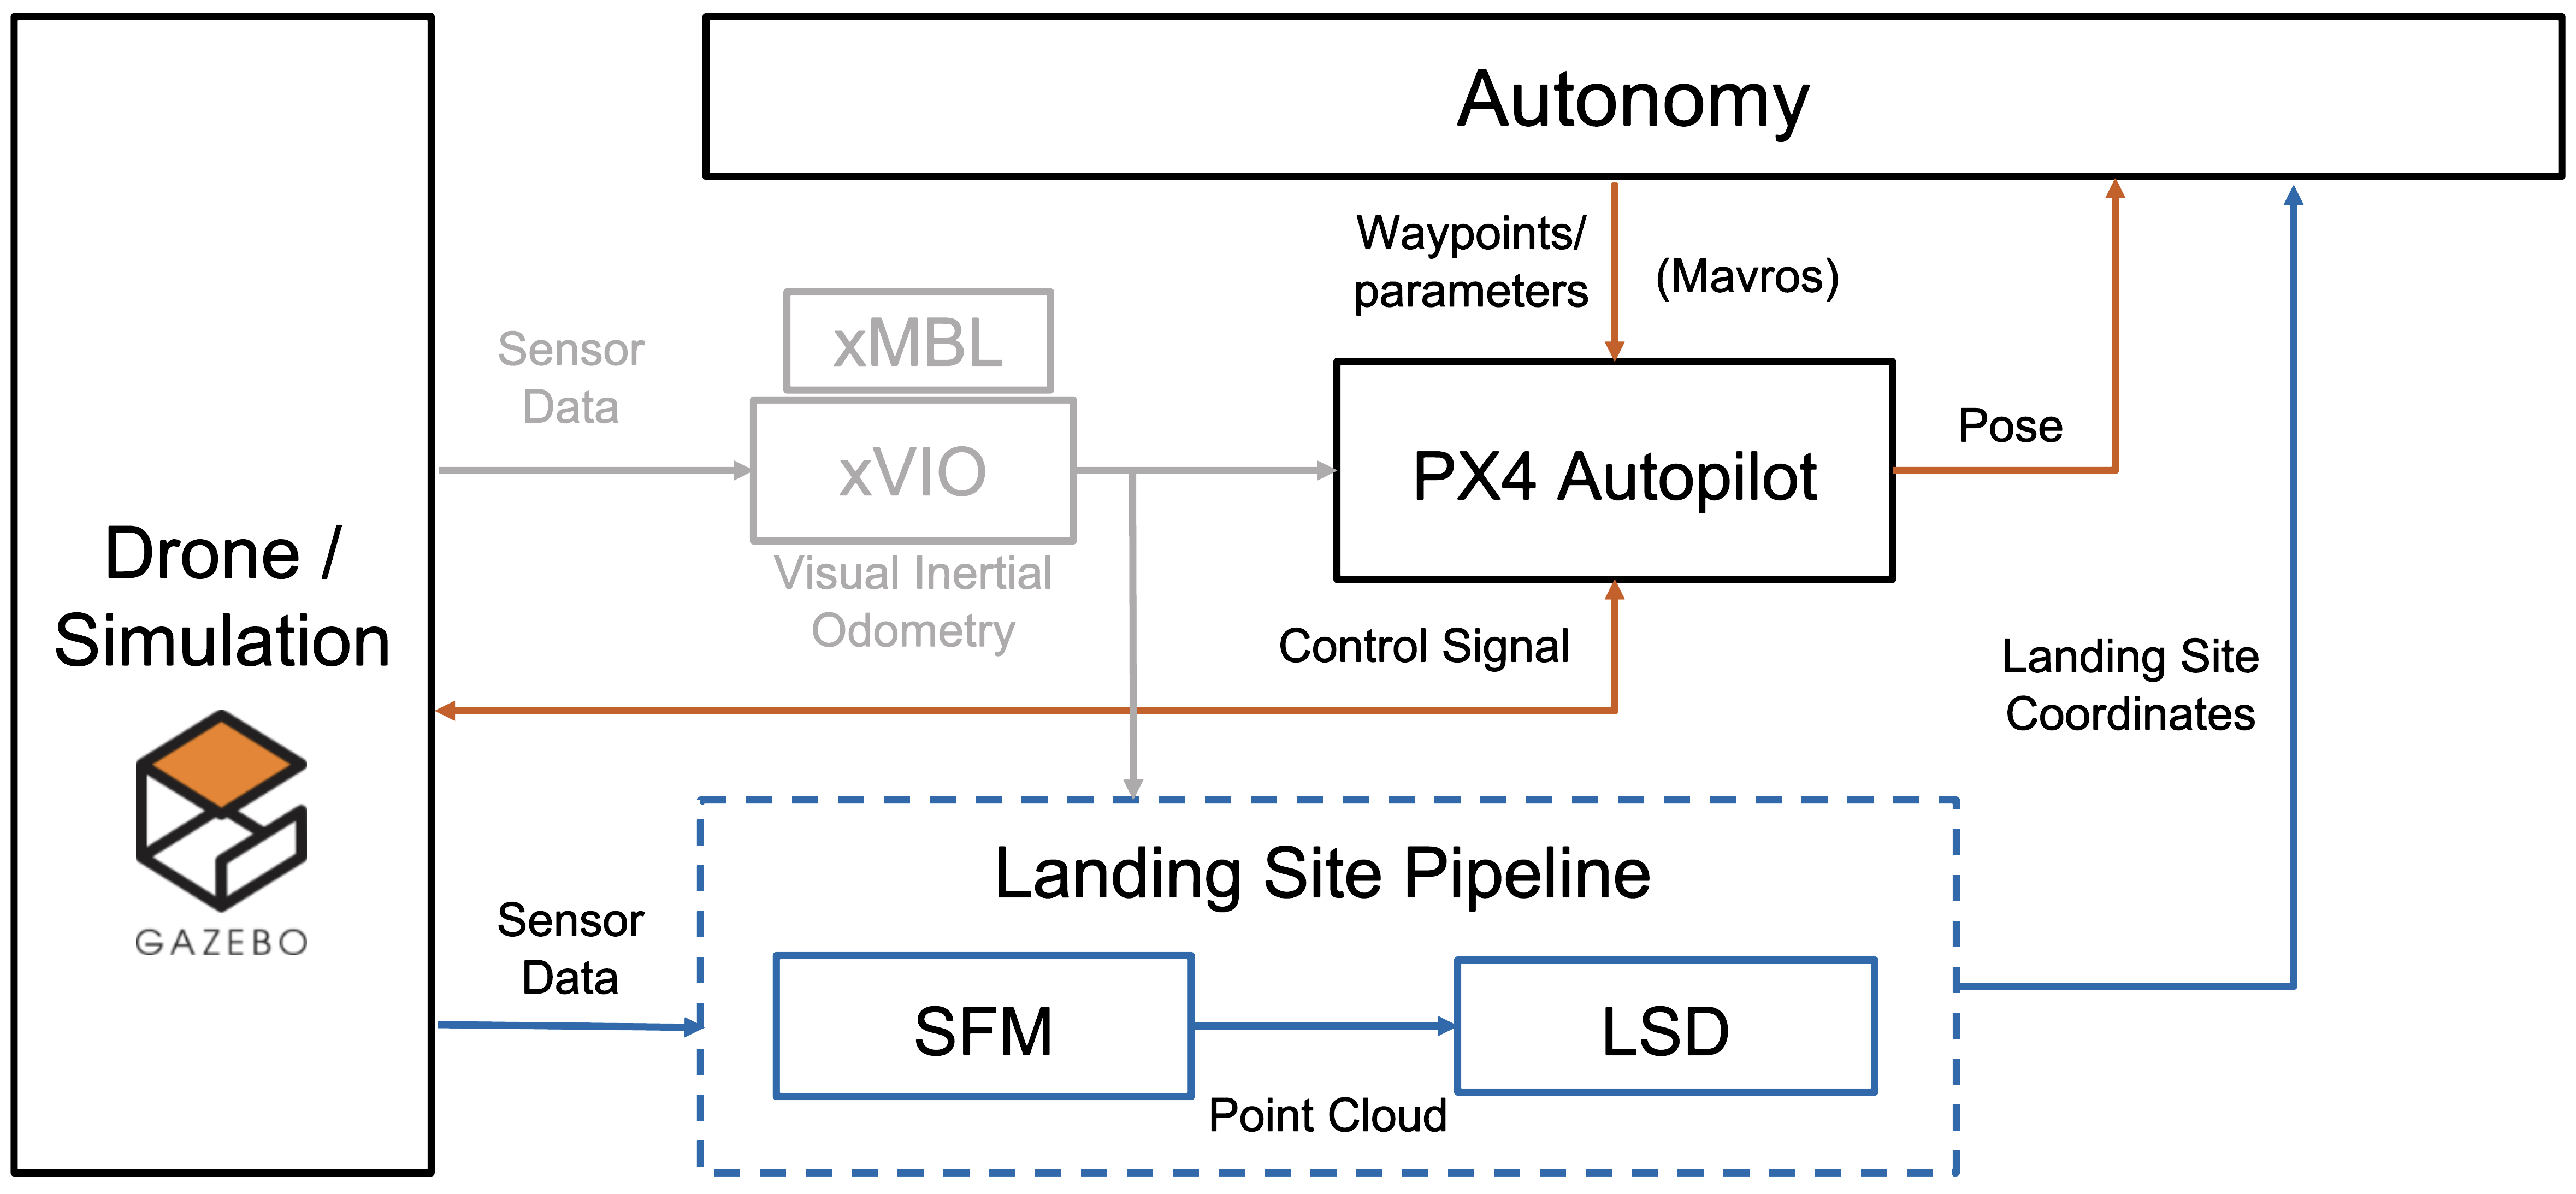
\includegraphics[scale=0.18]{images/setup/setup_flowchart.png}
    \caption{LORNA Project Setup}
    \label{fig:lorna_setup}
\end{figure}

As this thesis revolved around the combination of existing software instances, it is essential to display the individual parts comprising the LORNA project in more detail.

\clearpage %HERE
\section{Simulation}

Despite being able to deploy the landing site detection pipeline onto the voxl2 processor the majority of this thesis was done using a Gazebo Garden simulation of the drone. 

\begin{figure}[ht!]
    \centering
    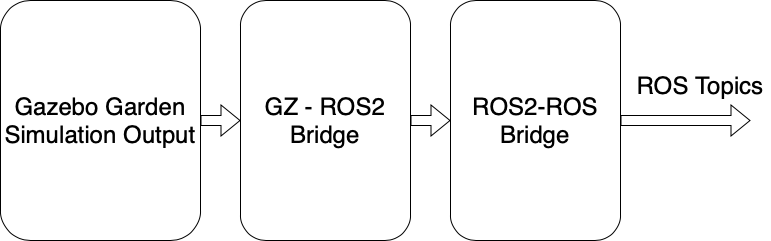
\includegraphics[scale=0.45]{images/setup/GZ_flowchart.png}
    \caption{Gazebo ROS Bridge}
\end{figure}


As the entire software stack of the LORNA project is dependent on ROS instead of ROS2 a bridge was used to convert the sensor information from Gazebo to ROS2 and from ROS2 to ROS.


\section{Landing Site Acquisition Pipeline}\label{sec:setup:LSD}

The landing site acquisition pipeline consists of two nodes. A structure from motion node \citep{SFM} which creates a pointcloud using a keyframe based stereo approach on monocular images and a landing site detector node \citep{LSD1, LSD2} which aggregates the depth measurements into a rolling buffer based multi-resolution depth map and segments landing sites on the created DEM. The found landing sites are then supplied to the autonomy. 

\subsection{Structure From Motion (SFM)}\label{subsec:setup:SFM}

\subsubsection{SFM - Bundle Adjustment}

\begin{figure}[ht!]
    \centering
    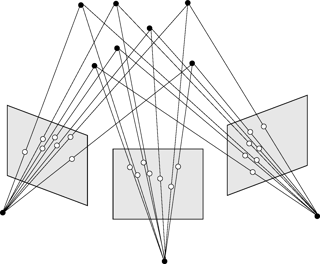
\includegraphics[scale=0.5]{images/setup/BA.png}
    \caption{Bundle Adjustment Procedure}
\end{figure}

In a first step the keyframes are filled with the incoming images and their respective camera pose information. Once the keyframes are filled, each iteration the input as well as all the keyframe poses are refined using a Bundle Adjustment algorithm. 

\subsubsection{SFM - Stereo Depth}

The keyframes and their refined poses are then compared to the new incoming image with regards to image overlap and feature retention. Chosing the most adequate keyframe and the incoming frame, one can create a depth image. The depth image is then converted into a pointcloud and packaged together with the respective poses of the images. This allows not only to correctly locate the points in a global frame but also to derive the baseline with which that pointcloud was created.

\subsubsection{SFM - Keyframe Updates}

At the end of an iteration the keyframes are updated based on the aforementioned characteristics of image overlap and feature retention quality.

\subsection{Landing Site Detection (LSD)}\label{subsec:setup:LSD}

\subsubsection{LSD - Depth Aggregation}

\begin{figure}[ht!]
    \centering
    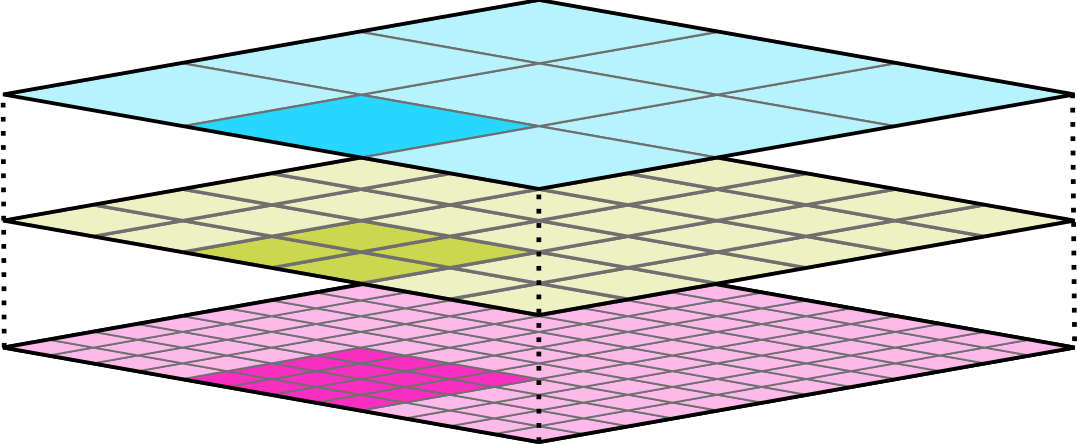
\includegraphics[scale=0.25]{images/setup/DEM.png}
    \caption{Multi Resolution Depth Map}
    \label{fig:DEM}
\end{figure}

The foundation of the landing site detection mechanism is a rolling buffer based multi resolution depth map as indicated in \cref{fig:DEM}. Each cell in this dense elevation map (DEM) contains an optimal mixture of gaussian (OMG) state as described in \citet{LSD2}. Each base layer cell is represented with 4 cells at a higher resolution layer.

Each point cloud input iteration, the measurements are placed in the respective cells based on the level of detail of the perceived points. In a subsequent step the measurements are pooled up and down the resolution layers in order to make the DEM more consistent and interpolate missing values.

One thing to note is that since the OMG variance decreases with an increased number of measurements, the cell values converge over time when receiving the same terrain information.

\subsubsection{LSD - Hazard Segmentation}

On the created depth map landing sites can then be detected. This is done using a roughness and slope assessment of the perceived terrain. Roughness defines the maximum absolute altitude difference around a cell in a certain resolution layer and slope is determined by fitting a plane to the vicinity of a considered point.

If the roughness and slope values lie within the acceptance threshold, the spot is recognized as a landing site and marked as such in a binary landing map. 

\begin{figure}[ht!]
    \centering
    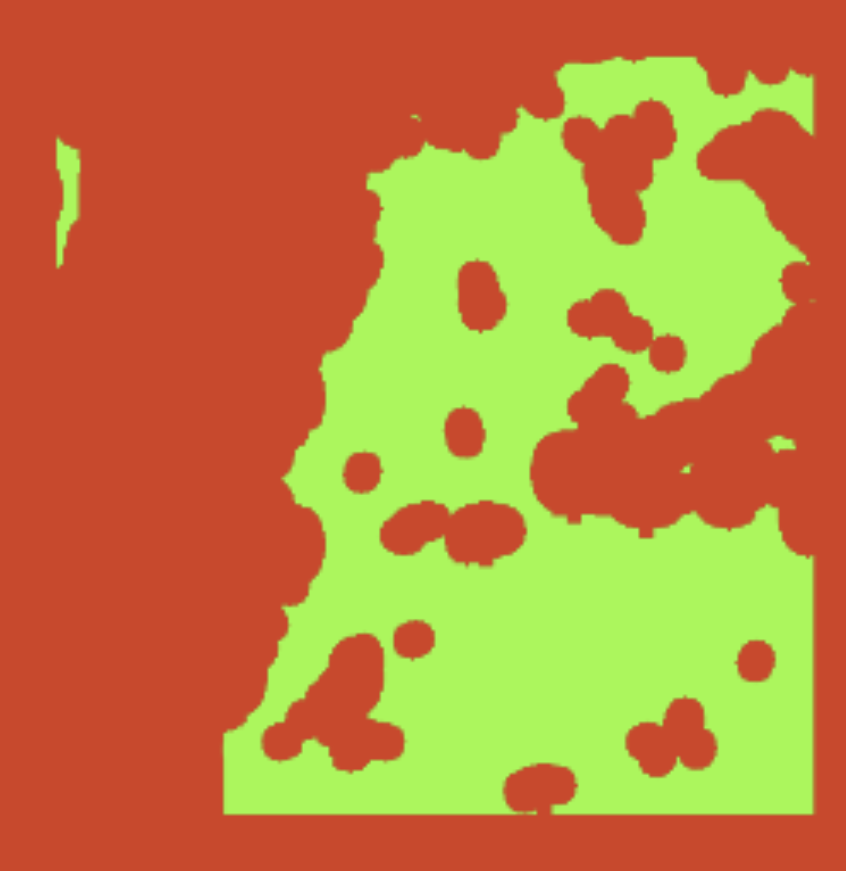
\includegraphics[scale=0.5]{images/setup/ls_map.png}
    \caption{Binary Landing Site Map}
    \label{fig:ls_map}
\end{figure}

\subsubsection{LSD - Landing Site Selection}

After applying a distance transform on the landing site map and performing non-maximum suppression on the landing site sizes, the biggest landing sites are found. Their positions are then refined one last time using a mean shift algorithm that considers roughness, uncertainty and size once again. 

\begin{figure}[ht!]
    \centering
    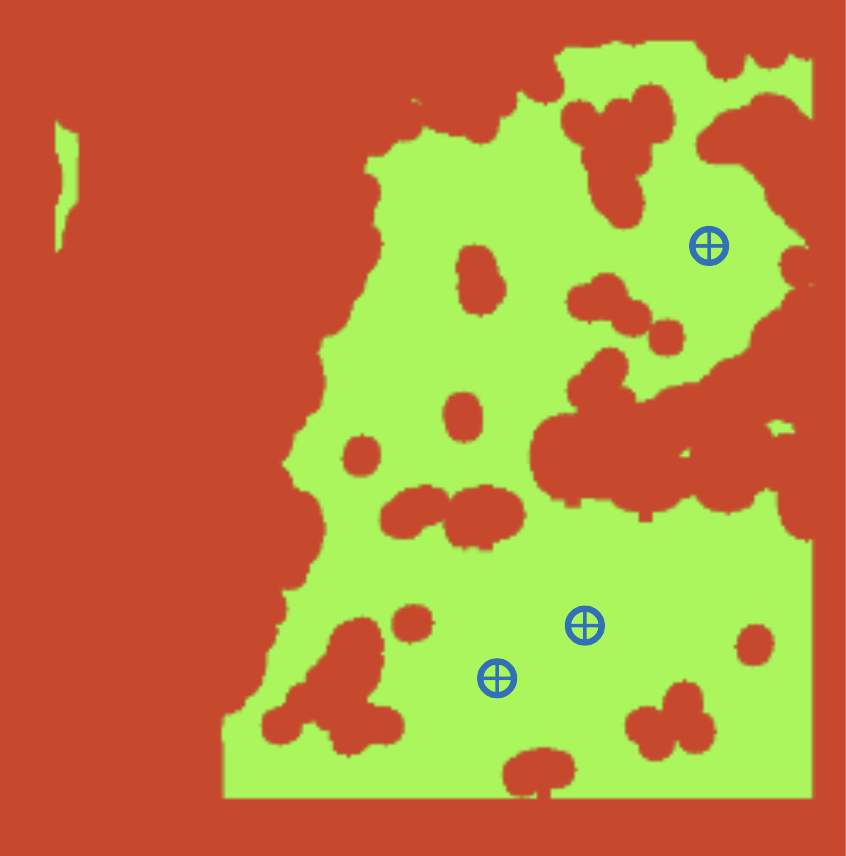
\includegraphics[scale=0.5]{images/setup/ls_map_nms.png}
    \caption{Binary Landing Site Map after Non Maximum Suppression}
    \label{fig:ls_map_nps}
\end{figure}

\clearpage %HERE

\subsubsection{LSD - Debug Images}

\begin{figure}[ht!]
    \centering
    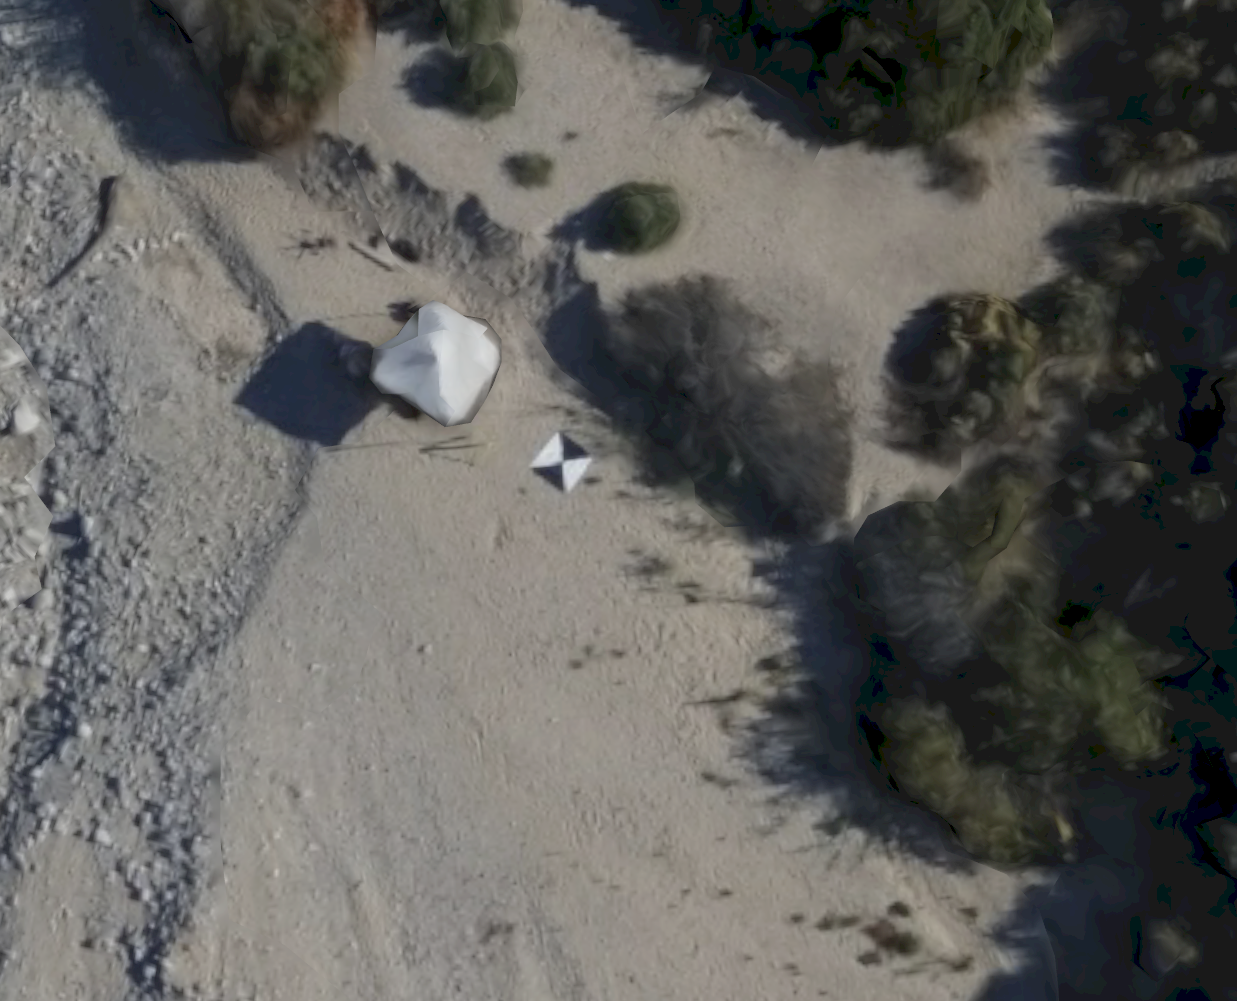
\includegraphics[scale=0.25]{images/setup/lsd_debug_reference.png}
    \caption{Gazebo Simulation Reference}
    \label{fig:lsd_debug_ref}
\end{figure}

\begin{figure}[ht!]
    \centering
    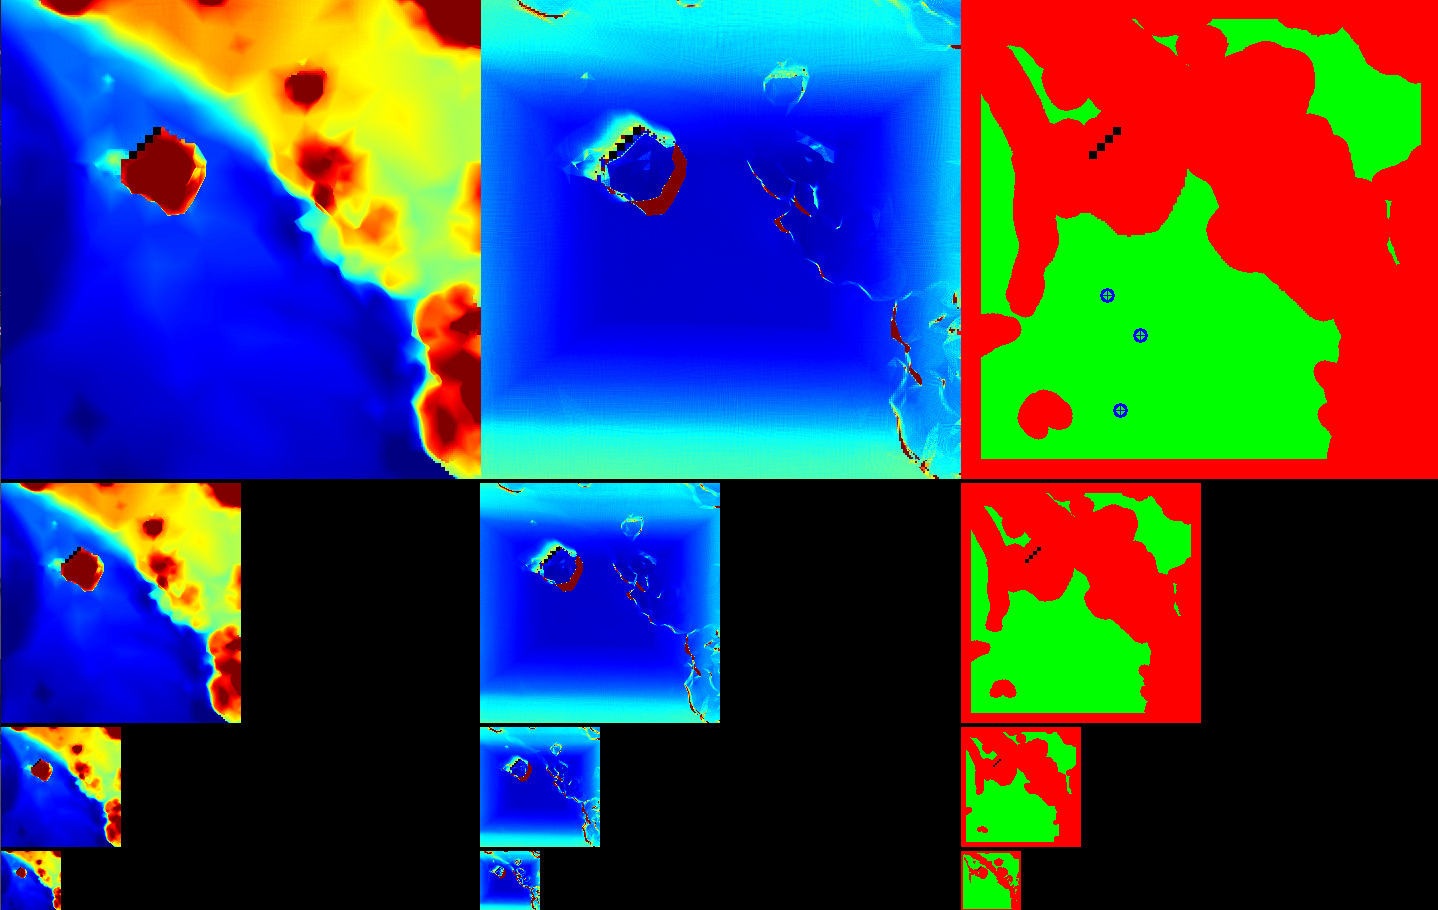
\includegraphics[scale=0.25]{images/setup/lsd_debug_image.png}
    \caption{LSD Debug Image - Left: DEM, Middle: Uncertainties, Right: LS Map}
    \label{fig:lsd_debug}
\end{figure}

The landing site detection debug image is a good comprehensive visualization of the landing spot detection procedure. 

On the left one can see the multi-resolution map displaying the same terrain area in different resolutions. Red pixels are closer, blue further away.

In the middle one can see the uncertainties of the detected points. For simplification purposes the variance of the detected points is simply the associated stereo depth error.

On the right is the above mentioned binary landing site map. Green indicates valid landing sites, and the blue crosses indicate the chosen non-max suppressed and mean shifted landing sites.

\section{Autonomy}\label{sec:setup:autonomy}

The autonomous framework was developed within the LORNA project. It is the overarching instance governing all the necessary behaviors and constituting the interface between all the different nodes of the process. It is connected to the flight controller through the Mavros wrapper of the Mavlink protocol. With this connection it can send waypoints and parameter updates to the flight controller.
In addition to the in \cref{fig:lorna_setup} shown connections it also communicates with a healthguard node keeping track of the systems health state and alerting in case of anomalies.

\begin{figure}[ht!]
    \centering
    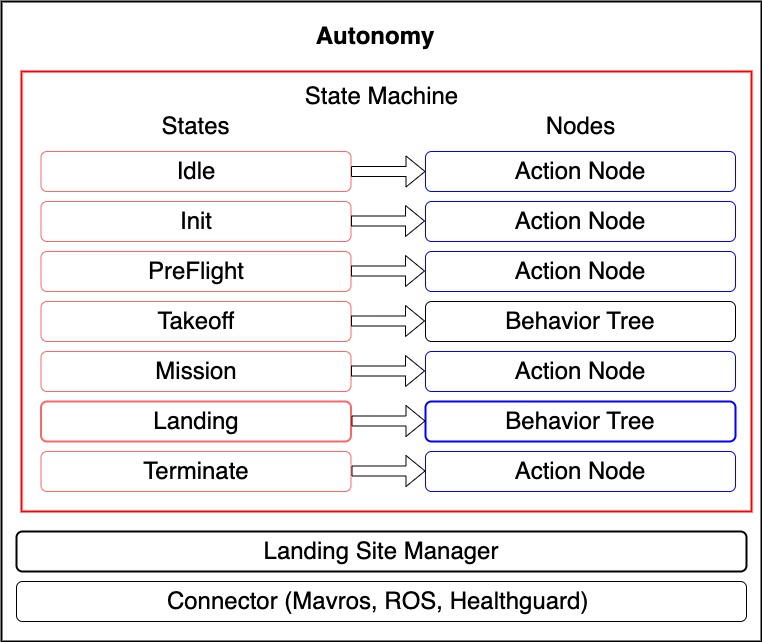
\includegraphics[scale=0.45]{images/setup/autonomy.png}
    \caption{Simplified Structure of the Autonomy}
    \label{fig:autonomy}
\end{figure}

The core of the autonomy is the state machine as depicted in \cref{fig:autonomy}. In each state the respective node is executed which most often is a single action node. For more complicated procedures a behavior tree is used. This is the case for the takeoff as well as landing nodes. As indicated in bold, the landing node is the most crucial node in this work as this is where the landing behavior using the landing sites is executed.

In a separate process the landing site manager processes incoming landing sites. The given setup before this thesis already had the template in place. Throughout this work I then replaced the dummy functionality of the landing site manager and the landing node with the final behaviors.

Lastly there the connector threads interact with the flight controller through Mavros and the ROS connector interacting with all the other nodes.








